For conference papers and journal papers, space constraints often dictate that your figures will have landscape aspect-ratios and sit at the top of a column of text.
In this dissertation format though, it is often desirable to have a full-page portrait shaped figure.
In this section, we give some examples of how to arrange this type of figure.

\subsection{More Subfig Trickery}
\begin{figure*}%
\centering%
\begin{tabular}{cc}%
\begin{tabular}{c}%
\subfloat[Distractor]{%
\label{subfig:distractorTexture}%
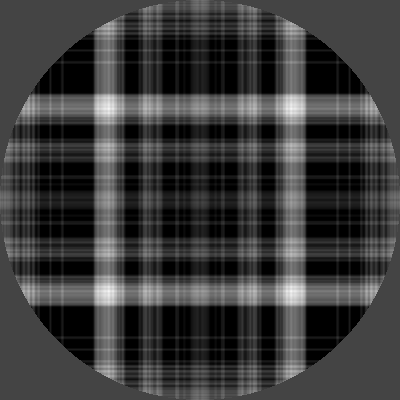
\includegraphics[width=80mm]{figures/distractorTexture}%
}\\%
\subfloat[Target]{%
\label{subfig:targetTexture}%
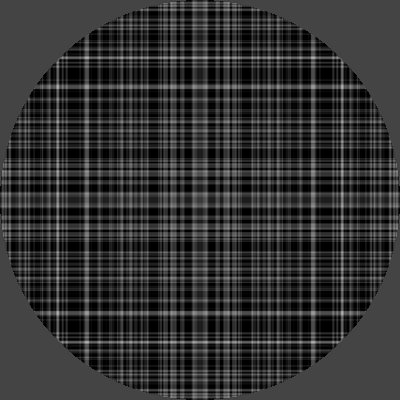
\includegraphics[width=80mm]{figures/targetTexture}%
}%
\end{tabular}%
\begin{tabular}{c}%
\captionsetup[subfloat]{labelformat=empty}%
\subfloat[]{%
\label{subfig:textureScale}%
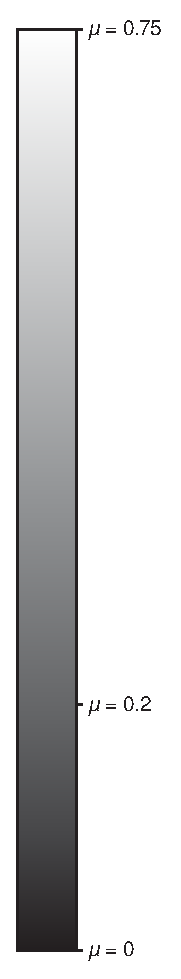
\includegraphics{figures/textureScale}%
}%
\end{tabular}%
\end{tabular}%
\caption[Scene element textures]{%
  Example \subref{subfig:distractorTexture}~distractor and \subref{subfig:targetTexture}~target texture patches at 2\ensuremath{\times} scale.
  The texture is represented visually by lightness corresponding to the coefficient of friction, $\mu$.
  The background surrounding both texture patches corresponds to the uniform coefficient of friction, $\mu_{background} = 0.2$.
  Note that although horizontal/vertical structure of the texture is readily apparent to the visual system, it is not perceived by haptic exploration.
}
\label{fig:sceneElementTextures}%
\end{figure*}%
In \autoref{fig:sceneElementTextures}, \texttt{tabular} environments are used to arrange three subfigures in a full-page figure (a \texttt{figure*}).
The caption for one of the subfigures is suppressed to make it seem like a legend.

\subsection{Side Captions}%
It is sometimes desirable to have a figure's caption somewhere other than below it.
This is particularly true for figures (or collections of subfigures) that are naturally tall and (relatively) narrow.
See, for example, \autoref{fig:profiles}.
The \texttt{floatrow} package helps make that possible.

% The floatrow package seems to have a bug in computing the correct box size when
% the _float_ size is given (or measured automatically).
% As a hack, we specify the _caption_ width as the columnwidth less the float width,
% and tell floatrow to let the float fill the remaining space
\newlength{\forceCaptionWidth}%
\setlength{\forceCaptionWidth}{\columnwidth}%
\addtolength{\forceCaptionWidth}{-4in}%
\addtolength{\forceCaptionWidth}{-1em}%
\thisfloatsetup{%
                capposition=beside,%
                capbesideposition={right,center},%
                floatwidth=sidefil,%
                capbesidewidth=\forceCaptionWidth,%
                capbesidesep=quad,%
               }%
\begin{figure}[p]%
\fcapside%
{%
  \subfloat[Full Stiffness]{%
    \label{subfig:fullStiffnessProfile}%
    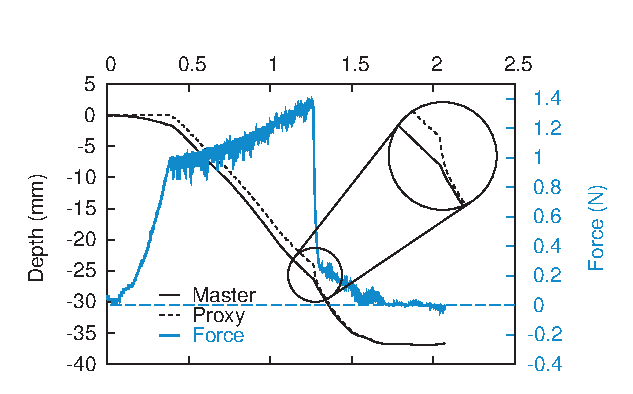
\includegraphics{figures/fullStiffnessProfile}%
  }\\%
  \subfloat[Degraded Stiffness]{%
    \label{subfig:degradedProfile}%
    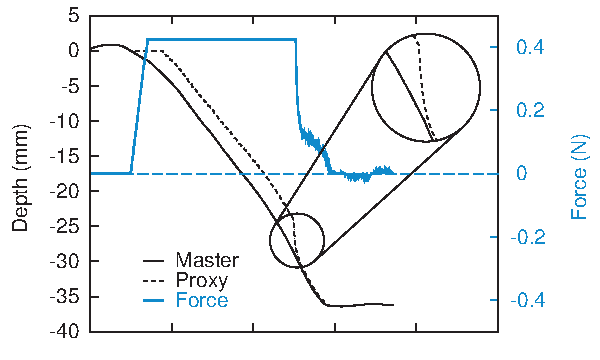
\includegraphics{figures/degradedProfile}%
  }\\%
  \subfloat[Augmented Low Stiffness]{%
    \label{subfig:augmentedProfile}%
    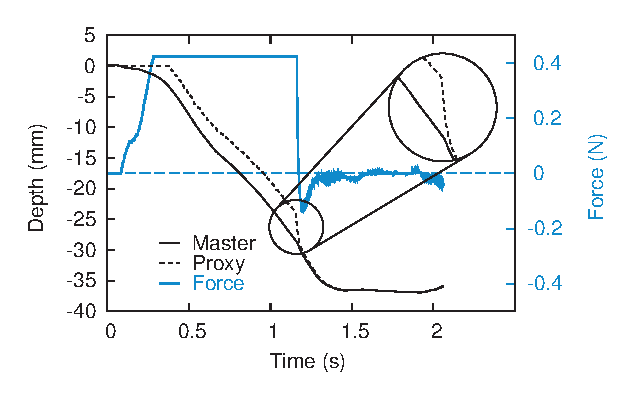
\includegraphics{figures/augmentedProfile}%
  }%
}%
{%
  %\captionsetup{justification=RaggedLeft,singlelinecheck=false}%
  \caption[Force/motion profiles for the different simulators]{%

  The force/motion profiles for the different simulators.

  \vspace{\baselineskip}%

  \subref{subfig:fullStiffnessProfile} The full stiffness simulator reproduces both the high-frequency force discontinuities encountered during carving, and the sudden negative acceleration of the master upon emergence from the material.

  \vspace{\baselineskip}%

  \subref{subfig:degradedProfile} The degraded stiffness simulator saturates below the force levels at which high-frequency discontinuities occur and fails to generate significant master acceleration at the point of emergence.

  \vspace{\baselineskip}%

  \subref{subfig:augmentedProfile} The open-loop force pulse applied in the augmented low stiffness simulator restores some of the master acceleration at the time of emergence from the material.}%
\label{fig:profiles}%
}%
\end{figure}%